\documentclass{article}
\usepackage[utf8]{inputenc}
\usepackage[T1]{fontenc}
\usepackage[francais]{babel}
\usepackage{amsmath}
\usepackage{graphicx}
\usepackage{color}
\usepackage{pdfpages} 
\usepackage{listings}
\usepackage{graphicx}
\usepackage{hyperref}
\usepackage{amsthm}
\usepackage{amssymb}
\usepackage{mathrsfs}
\usepackage{moreverb}
\usepackage{titletoc}
\usepackage{lmodern}
\usepackage{cubeDrawing}
\usepackage{lipsum}
\usepackage{bbold}

\definecolor{oxf}{RGB}{0, 33, 71}
\definecolor{or}{RGB}{239, 155, 15}
\definecolor{vert}{RGB}{135,167,103}
\definecolor{rouge}{RGB}{181,39,39}
\definecolor{violet}{RGB}{64,9,90}


\newcommand{\oxf}[1]{\textcolor{oxf}{#1}}

%Macros pour modifier la table des matières
\hypersetup{colorlinks=true, urlcolor=bleu, linkcolor=black}
\usepackage{hyperref}

\titlecontents{chapter}[20pt]% 103
   {\addvspace{1pc}\normalfont\sffamily\bfseries\large} 
            {\contentslabel[\thecontentslabel]{20pt}}{}{\hfill\contentspage}[] 
\titlecontents{section}[40pt]% 
   {\addvspace{0.6pc}\normalfont\sffamily} 
            {\contentslabel[\thecontentslabel]{25pt}}{}{\dotfill\contentspage}[] 
\titlecontents{subsection}[60pt]% 
   {\addvspace{0.3pc}\normalfont\sffamily} 
            {\contentslabel[\thecontentslabel]{25pt}}{}{\dotfill\contentspage}[]                            
\titlecontents*{subsubsection}[60pt]% 
   {\filright\normalfont\sffamily\footnotesize}{}{}{}[~{–}\ ][] 
\setcounter{tocdepth}{2}

\makeatletter\@addtoreset{section}{part}
\makeatother



%Page de garde
\makeatletter

\def\graphic#1{\def\@graphic{#1}}
\graphic{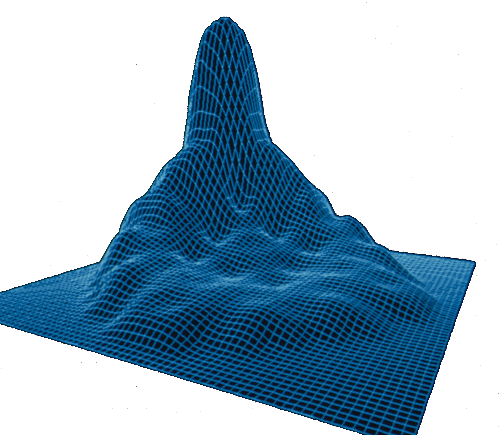
\includegraphics[scale=0.4]{logo.png}}
\def\clap#1{\hbox to 0pt{\hss #1\hss}}%
\def\ligne#1{%
\hbox to \hsize{%
\vbox{\centering #1}}}%
\def\haut#1#2#3{%
\hbox to \hsize{%
\rlap{\vtop{\raggedright #1}}%
\hss
\clap{\vtop{\centering #2}}%
\hss
\llap{\vtop{\raggedleft #3}}}}%
\def\bas#1#2#3{%
\hbox to \hsize{%
\rlap{\vbox{\raggedright #1}}%
\hss
\clap{\vbox{\centering #2}}%
\hss
\llap{\vbox{\raggedleft #3}}}}%
\def\maketitle{%
\thispagestyle{empty}\vbox to \vsize{%
\begin{tikzpicture}[remember picture,overlay]
\coordinate [below=2.5cm] (midpoint) at (current page.north);
\node [name=colourbar,
anchor=base,
fill=oxf,
minimum width=\paperwidth,
minimum height=1cm] at (midpoint){};
\node [
fill=oxf,
text = white,
xshift=2cm] at (midpoint){\Large{\textsf{Institut National des Sciences Appliquées de Rouen}}};
% Define the point where the logo will go
\coordinate [right=4cm] (logo) at (colourbar.west);
% Set coordinate system origin
\begin{scope}[shift=(logo)]
% Draw the outline
%\filldraw [white,draw=oxf] (2.3,0.85) -- (-2,0.85) -- (-2.8,-0.85) -- (2.3,-0.85) --cycle;
\filldraw [white,draw=oxf] (2.3,0.85) -- (-2.5,0.85) -- (-2.5,-0.85) -- (2.3,-0.85) --cycle;
\filldraw [oxf,draw=oxf] (-10,-24) -- (30,-24) -- (30,-23) -- (-10,-23) --cycle;
% Include the logo
\node {\includegraphics[width=4cm]{logoINSAdeRouen.jpg}};
\end{scope}
\end{tikzpicture}
\vspace{3cm}
%\usefont{OT1}{phv}{m}{n}
\begin{center}
\textbf{\huge \@title }
\end{center}
\vspace{1cm}
\par
\hrule height 4pt
\par
\vspace{0.5cm}
\begin{center}
\Large \@author
\par
\end{center}
\vfill
\begin{center}
\@graphic 
\end{center}
\vspace{1cm}
\haut{}{\@blurb}{}
\vspace{1cm}
\bas{}{\@date}{}
}
\cleardoublepage
}
\def\date#1{\def\@date{#1}}
\def\author#1{\def\@author{#1}}
\def\title#1{\def\@title{#1}}
\def\location#1{\def\@location{#1}}
\def\blurb#1{\def\@blurb{#1}}
\makeatother


\date{\today}
\title{Résolution numérique des équations de Saint-Venant par la méthode des éléments finis}
\author{Gabrielle Collette, Alexandre Vieira \& Conrad Hillairet}
\vfill
\blurb{
\textbf{Rapport}\\[1em]
Professeur référent : Christian Goût\\
}

%\usepackage[8pt]{extsizes}

\hypersetup{colorlinks=true, urlcolor=bleu, linkcolor=red}

%Def = Definition
%Theo = Théorème
%Prop = Propriété
%Coro = Corollaire
%Lem = Lemme

\makeatletter
\@addtoreset{section}{part}
\makeatother

\begin{document}

\setcounter{tocdepth}{4}
\tableofcontents
\newpage

\part{Signal}
\begin{enumerate}
\item Définition d'une moyenne, d'une correlation
\item Expression de la covariance
\item Définition de WSS
\item Définition d'ergodique
\item Densité spectrale de puissance, lien avec correlation et moyenne par TF
\item Intercorrelation entre deux sorties en fonction de l'entrée
\item 
\end{enumerate}

\part{Optimisation combinatoire}
\begin{enumerate}
\item Définition d'un problème d'optimisation, de décision
\item Propriété entre problème d'optimisation et de décision
\item Ensemble des énoncés de $\Pi$ codés par $c$ pour lesquels la réponse est oui
\item Condition pour qu'un programme sésolve $\Pi$
\item Définition d'une complexité
\item Algorithme polynomial, problème polynomial
\item Définition de P et $\mathcal{P}$
\item Fonction calculée par A
\item Fonction calculable polynomialement
\item MT non déterministe : temps de calcul, temps de reconnaissance de $x$
\item Algorithme non déterministe polynomial (NP)
\item Définition de $\mathcal{N}\mathcal{P}$
\item $\mathcal{P}\subset\mathcal{N}\mathcal{P}$
\item Compléxité algorithme d'un problème $\mathcal{NP}$
\item Définition d'une réduction polynomiale, notation
\item Propriété sur l'appartenance à $\mathcal{P}$ si réduction polynomiale
\item Transitivité
\item Définition de polynomialement équivalent
\item Plus petite classe d'éqivalence pour $\alpha$
\item Classe $\mathcal{NP}$-complet
\item Théorème de Cook
\end{enumerate}

\part{EDP}
\begin{enumerate}
\item Définition de l'ordre
\item Formule d'intégration par partie, formules de Green.
\item Classification des EDP : elliptiques, paraboliques, hyperboliques
\item Conditions de Dirichlet et de Neumann
\item Différence finies : approximation de la dérivée
\item Définition d'approximation consistante d'ordre p
\item Lemme : approximation de la dérivée seconde
\item Définition erreur de consistance, schéma consistant au sens d'une norme, schéma consustant d'ordre p
\item Définition normes matricielles subordonnées 1, 2 et $\infty$
\item Définition de vecteur et matrice positif(ve)
\item Définition matrice monotone
\item Lemme : équivalence matrice monotone
\item 
\end{enumerate}

\part{Calcul spectral}
\begin{enumerate}
\item Produit scalaire 2 vecteurs propres
\item Définition deux matrices semblables, propriété des éléments propres pour les matrices propres
\item Algorithme de la puissance itérée
\end{enumerate}

\part{Réseau}
\begin{enumerate}
\item 
\end{enumerate}

\part{Finance}
\begin{enumerate}
\item Agent économique : qui supporte un besoin et qui dégage une capacité ?
\item Financement intermédié
\item Définition de marché, marché des capitaux. Titres, émetteurs
\item Marchés monétaires et financiers. Actions, Obligations. Marché primaire, secondaire.
\item Politique monétaire. 
\item Membres zone euro. 2 définitions des autorités monétaires
\item Objectif de la BCE.
\item Panier. Inflation en France et en Europe en janvier 2013
\item Qu'est-ce qui fait monter l'inflation ?
\end{enumerate}
\end{document}
